\section{实验一\ 初识实验环境}

\subsection{实验目的}

\begin{enumerate}
	\item 安装好实验环境,熟悉基本操作
	\item 掌握包括 objdump、makefile、QEMU、Bochs 等实验工具的基本用法
\end{enumerate}

\subsection{NEUOS 实验环境}

本实验环境是安装了内核开发工具的 Manjaro GNOME Edition (17.1.11) 虚拟机镜像。在 Windows 或 Linux 上安装 VirtualBox,然后下载该虚拟机镜像(约 2.5 GB)\footnote{百度网盘链接:\url{https://pan.baidu.com/s/1agqKofK4zD-vMlw4uykplg},密码:7375}。

在 VirtualBox 菜单栏中点击“管理 - 导入虚拟电脑”以导入该镜像。推荐使用该镜像以避免繁琐的安装以及可能存在的依赖问题。另外也可自行在 Linux 环境中安装以下工具作为实验环境:git、gcc、gdb、make、qemu、bochs.

实验环境中的 oshacker 账户的默认密码是 “oshacker” 。
若在 Ubuntu 下使用 VirtualBox 启动虚拟机镜像时,出现 “kernel driver not installed” 的错误提示,访问此处 \footnote{\url{https://askubuntu.com/questions/760671/could-not-load-vboxdrv-after-upgrade-to-ubuntu-16-04-and-i-want-to-keep-secur}}。
若虚拟机运行不流畅,可在 VirtualBox 设置中调整内存大小、显存大小及处理器数量。
进入实验环境后,虚拟机的显示比例或许不正常,尝试在 VirtualBox 的“显示”设置中修改缩放率,或在 Manjaro 中修改显示设置。在桌面上右击,选择 Display Settings 即可。

不建议将系统语言设置为中文,某些软件可能出现乱码,并且在调试程序时使用英文调试信息在搜索引擎中检索是必要的。

启动虚拟机需要开启 VT-x 功能,可在 BIOS 中设置\footnote{\url{https://jingyan.baidu.com/article/8ebacdf0df465b49f65cd5d5.html}}。如果不支持 VT-x,您的电脑无法使用虚拟机。

\begin{figure}[htbp]
    \centering
    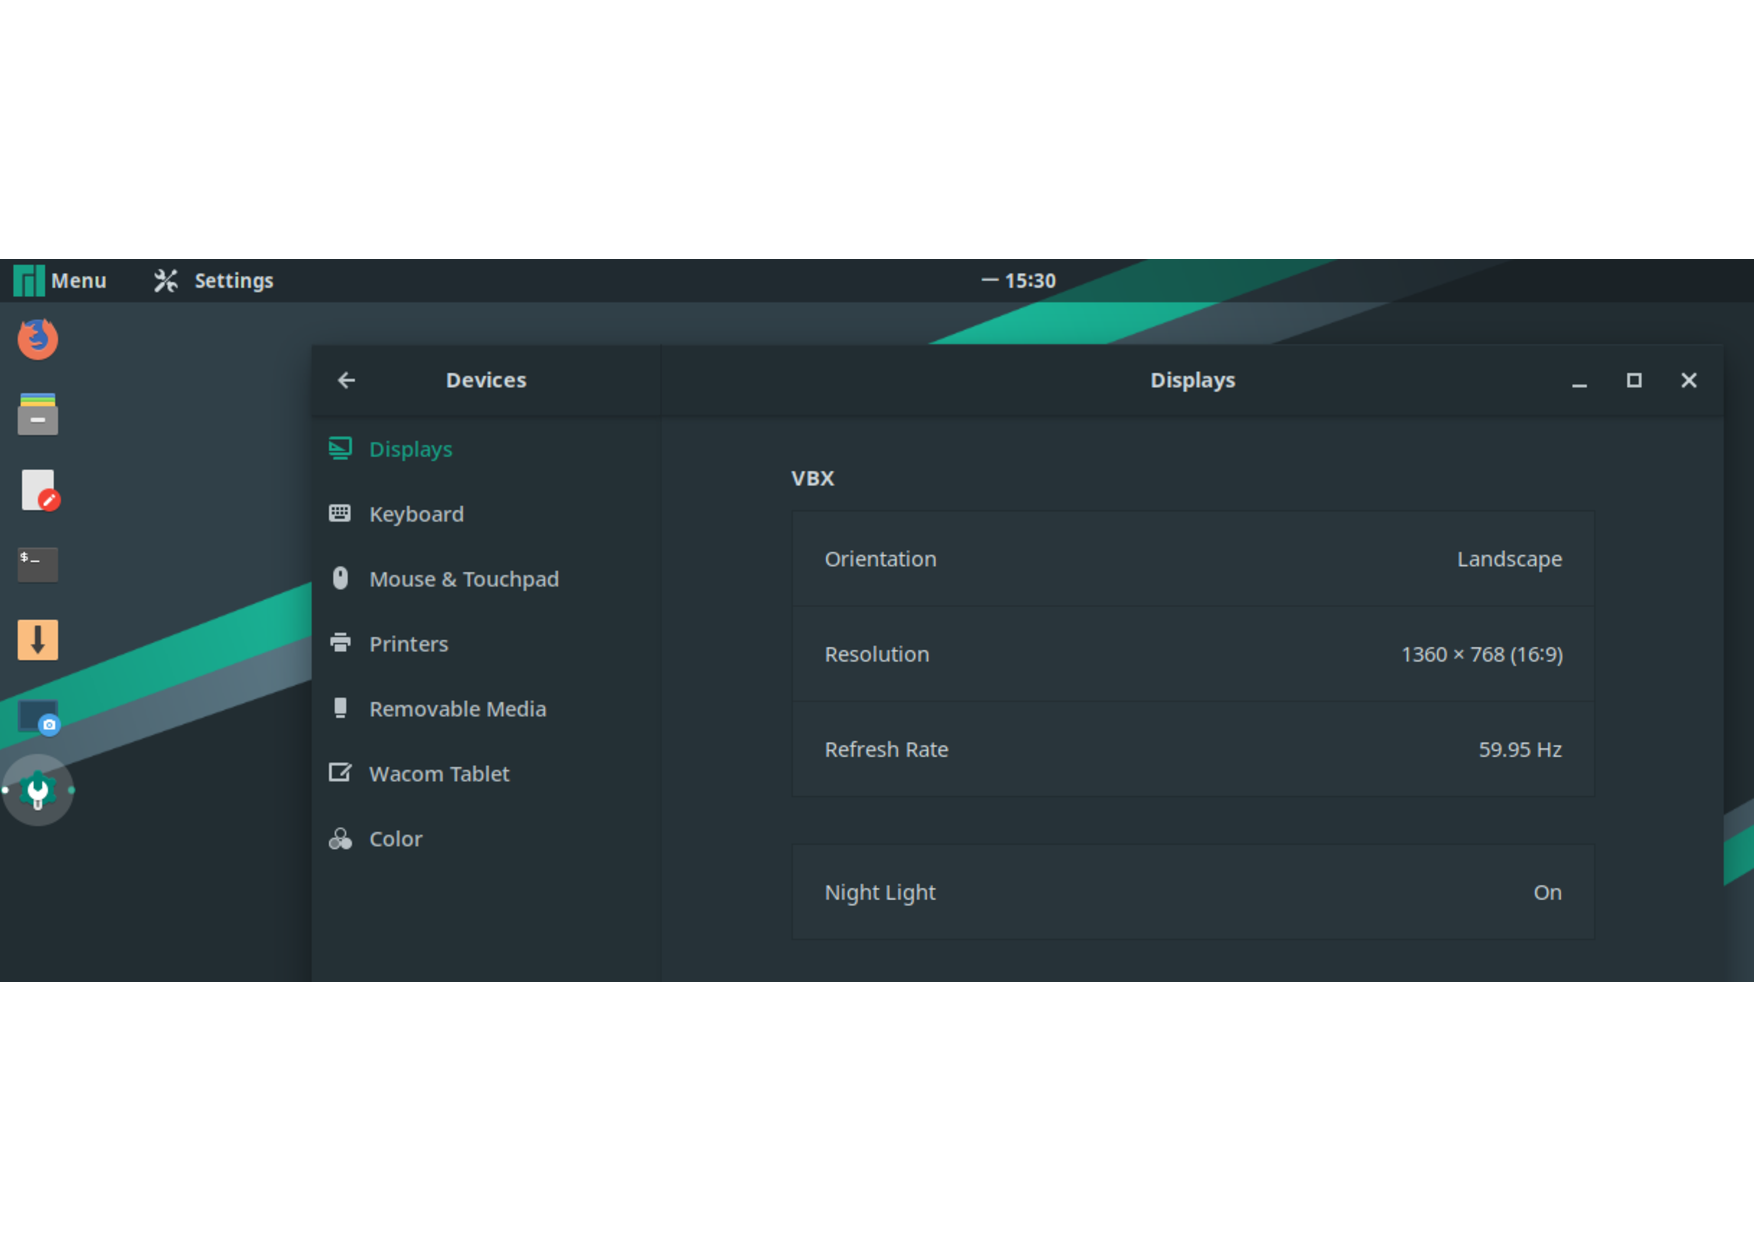
\includegraphics[width=\textwidth]{img/ManjaroDisplaySettings}
    \caption{Manjaro Display Settings}
    \label{fig:Manjaro Display Settings}
\end{figure}

NEUOS Lab Environment 的桌面是空白的,但它已包含实验所需的必要工具 GCC, GNU Toolchain, dd, Makefile, Bochs, QEMU 等。左侧 Dock 栏是常用软件。点击左下角按钮可查看应用列表。

打开 Files,\textbf{实验材料} “neuos-material” 位于 Documents 目录中。为确保实验材料是最新版本,进行所有实验前请打开终端,使用 cd 切换到 neuos-material 目录内,保证虚拟机联网状态,键入"git pull"拉取最新版。

GCC (GNU Compiler Collection) 是由 GNU 开发的编程语言编译器,支持的语言包括 C 语言。它是以 GPL 许可证所发行的自由软件,也是 GNU 计划的关键部分。GCC 原本作为 GNU 操作系统的官方编译器,现已被大多数包括 Linux 的类 Unix 操作系统采纳为标准的编译器。

Objdump 是显示二进制文件信息的工具。
dd \footnote{了解 dd 命令:\url{https://www.ibm.com/support/knowledgecenter/zh/ssw_aix_71/com.ibm.aix.cmds2/dd.htm}}的用途为转换和复制文件。
make 是一个工具程序,用于简化重复编译和重复链接进程。Makefile\footnote{学习 Makefile:\url{https://seisman.github.io/how-to-write-makefile/overview.html}}是由 make 程序引用的文本文件,它描述了目标的构建方式,并包含诸如源文件级依赖关系以及构建顺序依赖关系之类的信息。

\begin{mdframed}[hidealllines=true,backgroundcolor=gray!20]
\textbf{练习 } 尝试纠正 Makefile 文件 exp1/Makefile 中的错误,找到错误并解释其错误原因,其中至少有 3 处\textit{参数错误}或\textit{语法错误},其中一个错误与 gcc 优化参数有关。

在改正错误后,你可能需要实际验证该 Makefile 是否正确。任意编写一段可正常运行的的 C 程序,命名为 hello.c,作为被编译的源代码。在 exp1 目录下使用终端,键入 make,测试可执行文件能否正常地通过该 Makefile 生成、生成的可执行文件能否正常运行。
\end{mdframed}

\begin{mdframed}[hidealllines=true,backgroundcolor=gray!20]
\textbf{练习 }exp1/binary 程序可以在屏幕上打印一串字符,但在此之前用户需要输入正确的密码。请通过查阅文档了解 objdump 的用法,使用 objdump 程序查看二进制文件 exp1/binary 的 section 信息。其中有一个 section 为 “The password is ...”,请找到该密码,并运行 binary 输入密码,使程序打印字符串。

请解释你如何通过 objdump 查看二进制文件的 section 信息,并展示其中的密码与 binary 打印的字符串。
\end{mdframed}

\begin{figure}[htbp]
    \centering
    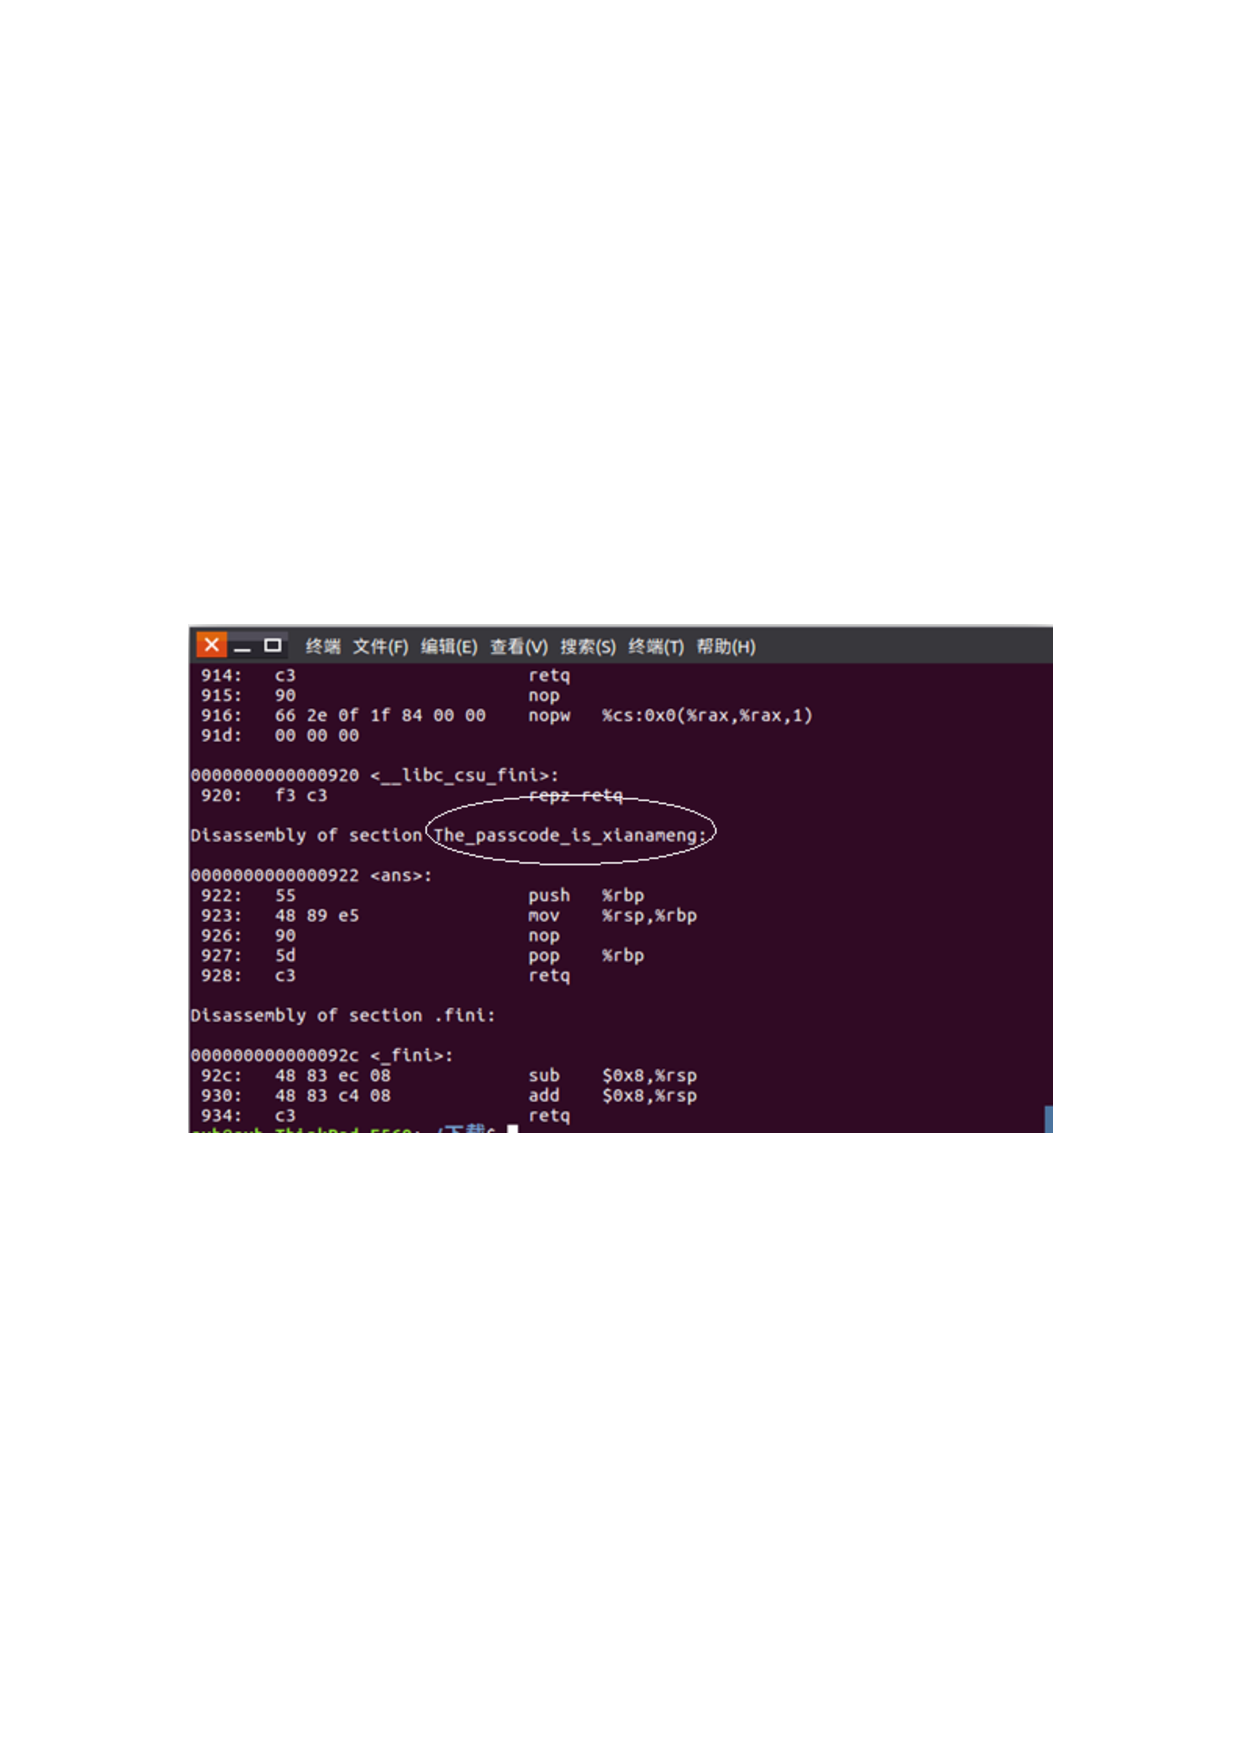
\includegraphics[width=\textwidth]{img/objdump查看section示例.pdf}
    \caption{objdump 查看 section 示例}
    \label{fig:objdump 查看 section 示例}
\end{figure}

\subsection{Bochs}

Bochs 是一种 x86 PC 仿真器和调试器。它提供对整个 PC 平台的仿真\footnote{使用 Bochs 进行平台仿真:\url{https://www.ibm.com/developerworks/cn/linux/l-bochs/index.html}},包括一个或多个处理器和各种不同的 PC 外围设备。Bochs 提供的并不是现代意义上的虚拟化,而是模拟。

\begin{figure}[htbp]
    \centering
    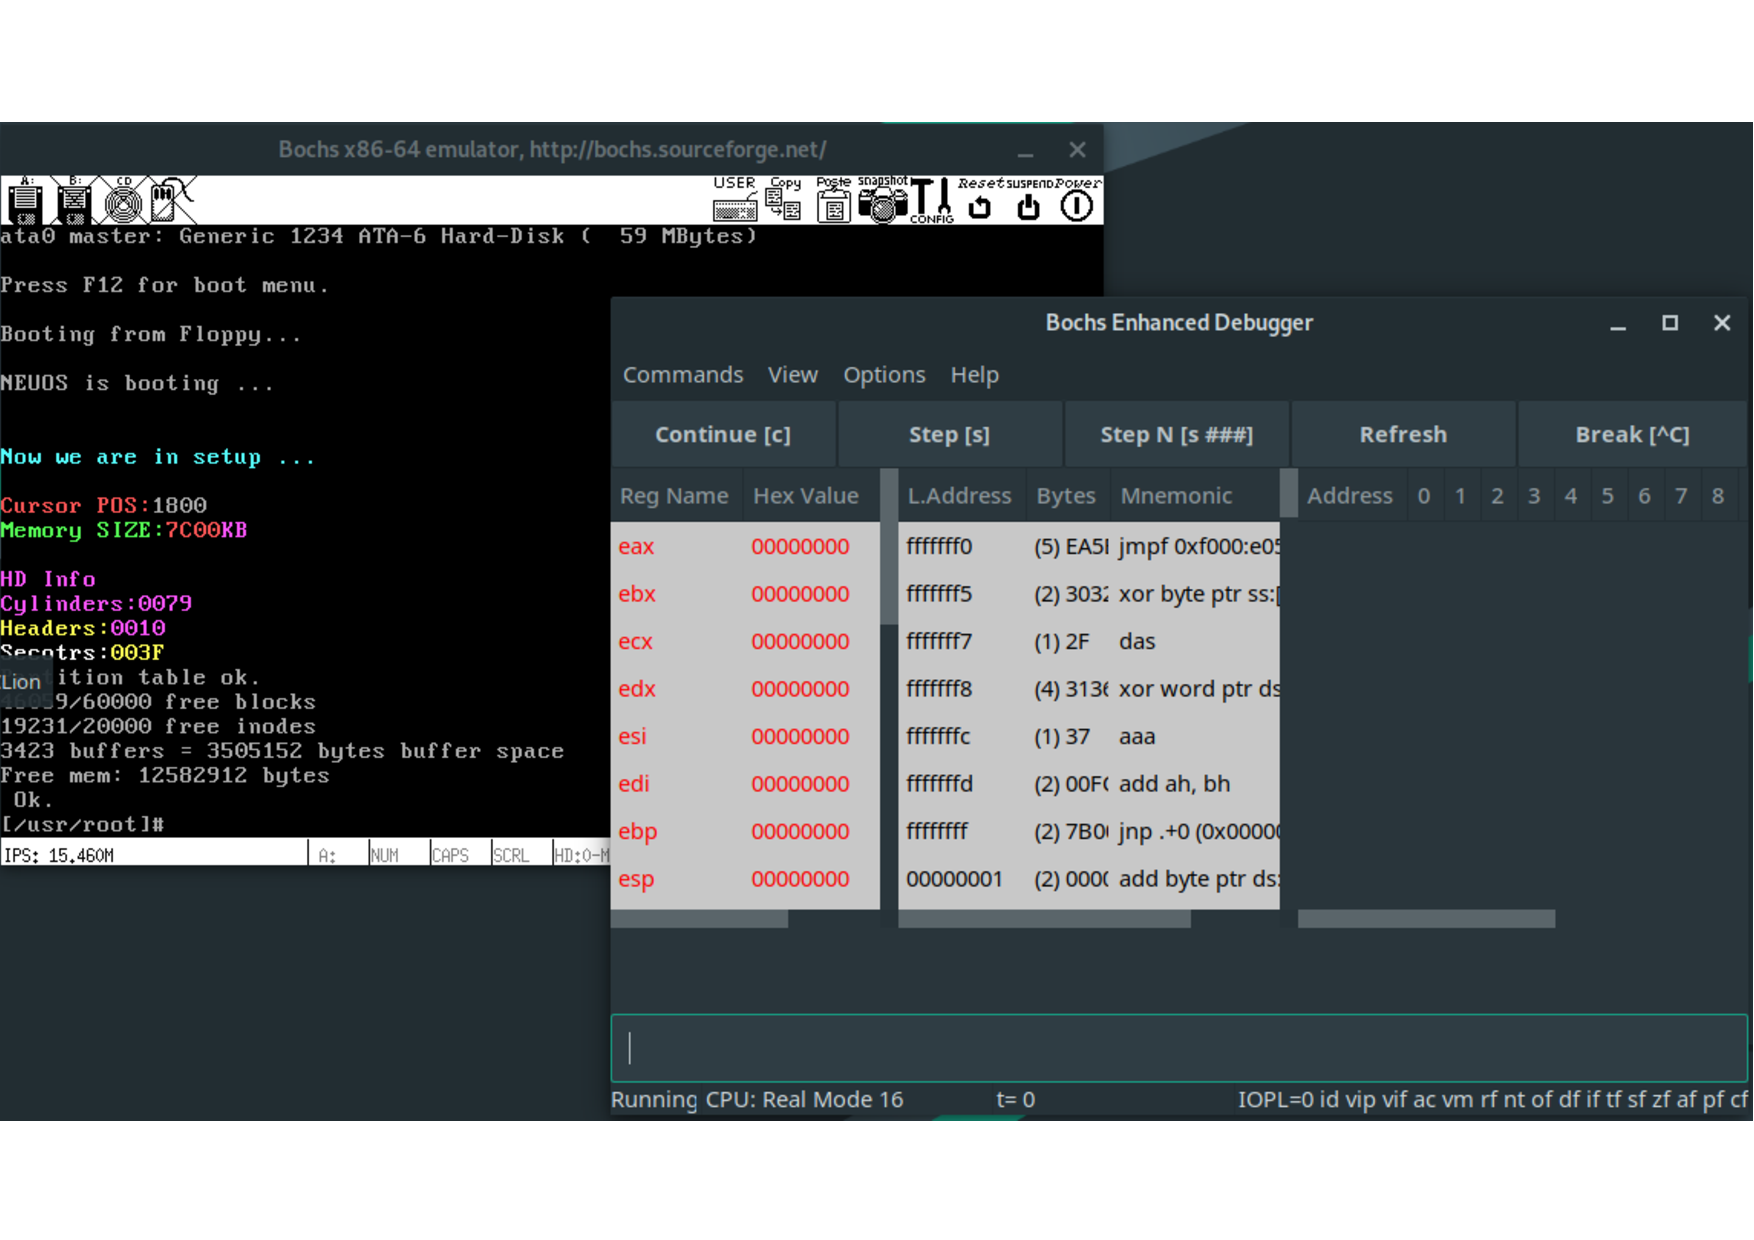
\includegraphics[width=\textwidth]{img/Bochs调试界面.pdf}
    \caption{Bochs 调试界面}
    \label{fig:Bochs 调试界面}
\end{figure}

Bochs 模拟器的启动需要配置文件,如 neu-os 目录下已写好的 bochsrc。要在 Bochs 中启动 NEUOS,启动命令行,打开 neu-os 目录,键入

\begin{lstlisting}
    make
    bochs -q
\end{lstlisting}

或者直接键入

\begin{lstlisting}
    make run_bochs
\end{lstlisting}

run\_bochs 命令定义在 Makefile 中。Bochs 会读取 bochsrc 的配置信息,启动模拟器。执行该命令后,在虚拟机中,终端和 bochs 界面可能重叠在显示屏幕上,你可能需要留意 bochs 界面是否已经启动。

如图 \ref{fig:Bochs 调试界面} 中的 Bochs Enhanced Debugger 窗口是 Bochs 的调试器,左侧是寄存器信息,中间是将执行的汇编代码,右侧用于显示地址信息。顶部的 Continue 按钮会使模拟器一直执行代码,直到发生错误、遇到断点或等待用户操作;Step 按钮会向下执行一步,Step N 按钮会向下执行指定步数。调试器的底部是 Bochs 的命令行。点击顶部菜单栏中的 View,可查看 GDT、IDT 等信息。图 \ref{fig:Bochs 调试界面} 中的 Bochs x86-64 emulator 是模拟器的运行窗口。

\begin{mdframed}[hidealllines=true,backgroundcolor=gray!20]
\textbf{练习 } 尝试在 Bochs 中启动 NEUOS,NEUOS 源码位于 NEUOS Lab Environment 的 Documents 目录下。

在 Bochs 中启动 NEUOS 时,在线性地址 0x000f7b14 处设置断点,查看调试信息。请阐述你如何在 Bochs 中设置与删除断点,并展示 Bochs 运行至断点时的截图。运行到断点后,Bochs 又如何继续执行指令?
\end{mdframed}

\begin{figure}[htbp]
    \centering
    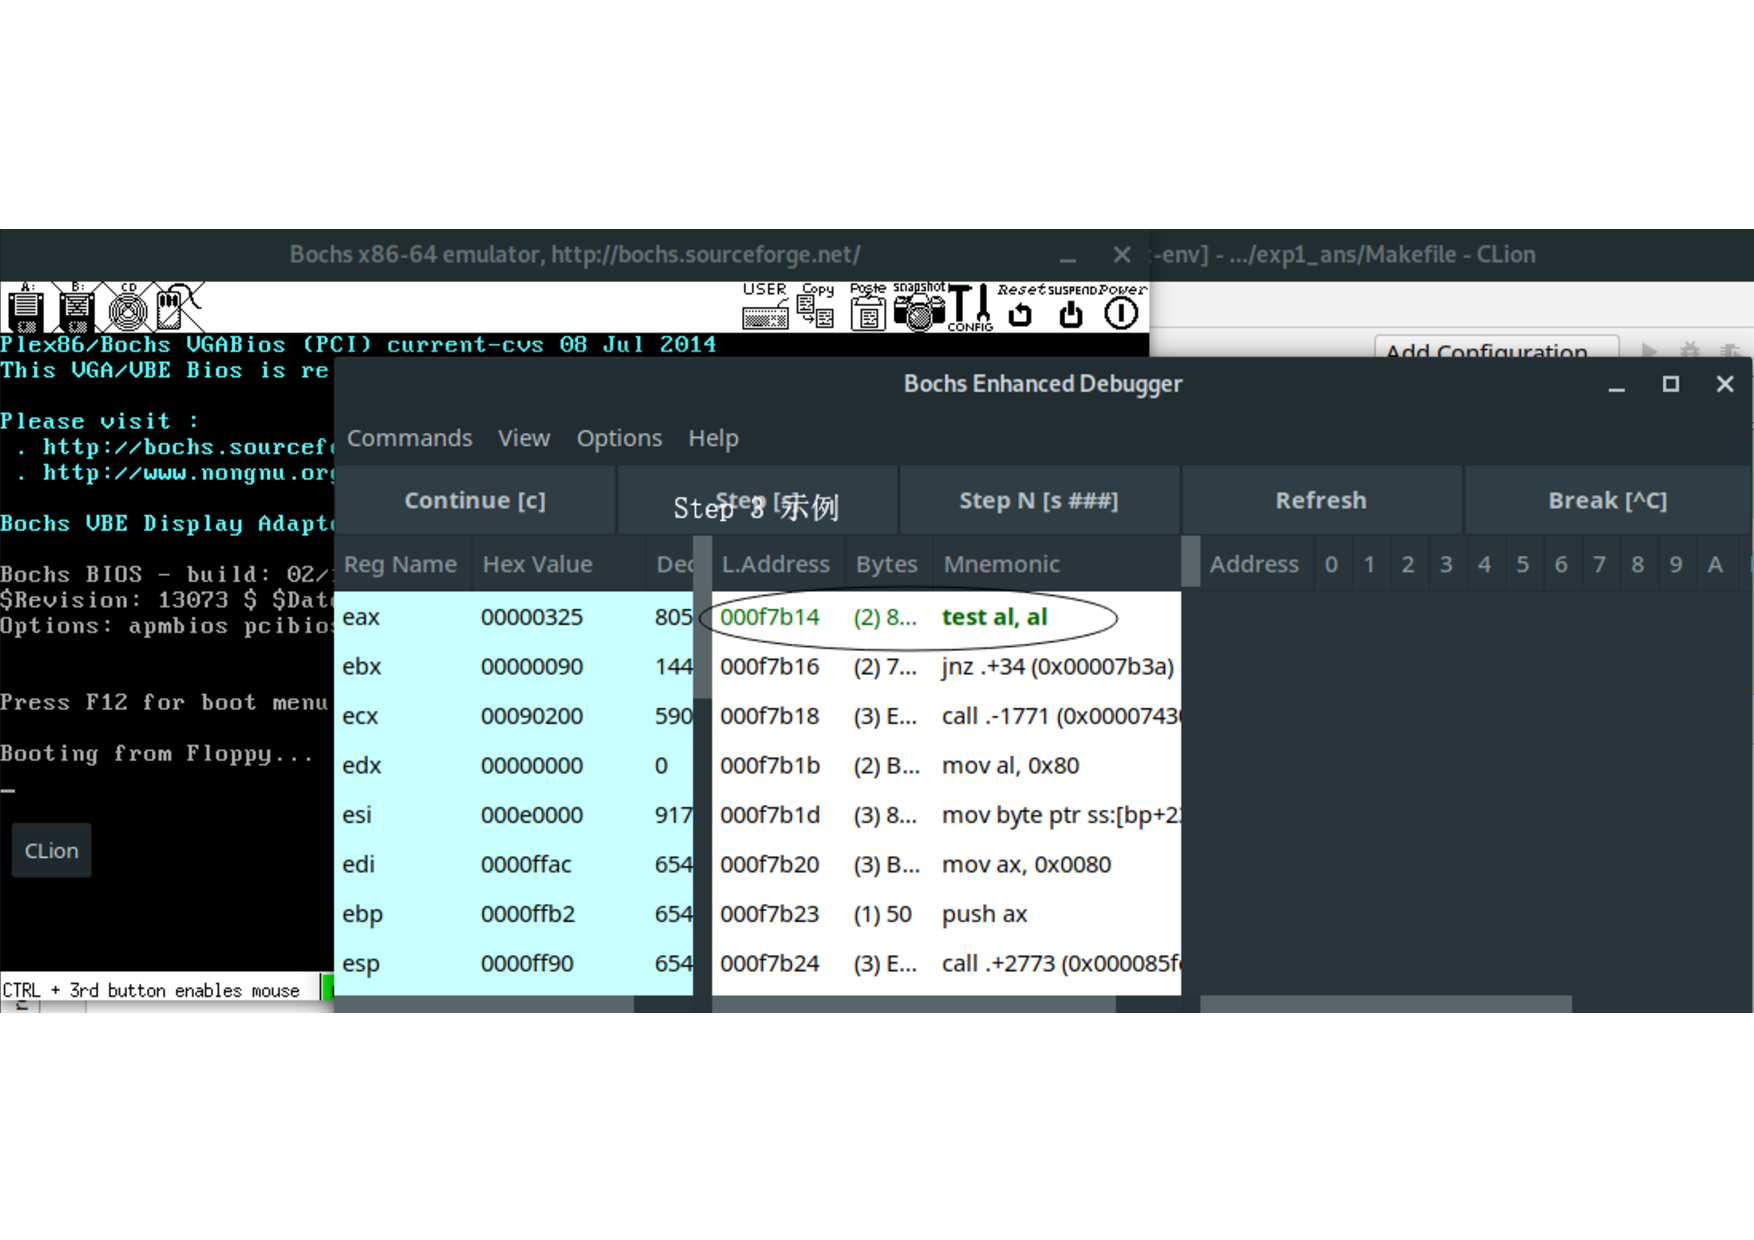
\includegraphics[width=\textwidth]{img/Bochs运行至断点.pdf}
    \caption{Bochs 运行至断点}
    \label{fig:Bochs 运行至断点}
\end{figure}

\subsection{QEMU}

与 Bochs 类似,QEMU \footnote{使用QEMU进行系统仿真:\url{https://www.ibm.com/developerworks/cn/linux/l-qemu/}}是一个面向完整 PC 系统的开源仿真器,它允许实现高级概念上的仿真,如对称多处理系统和其他处理器架构。

\begin{figure}[htbp]
    \centering
    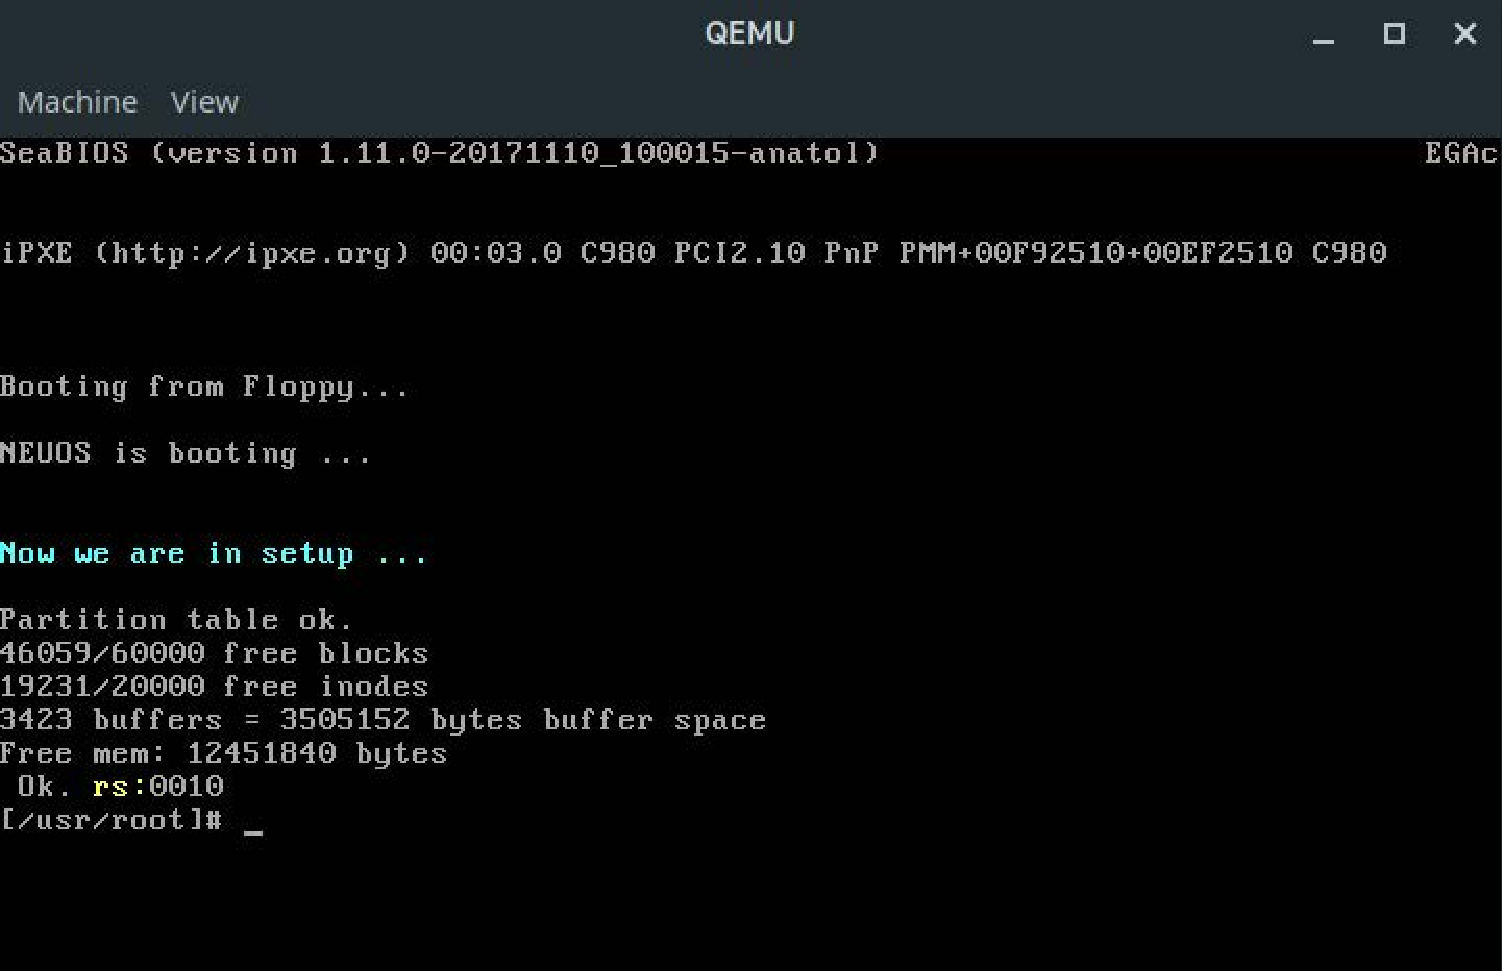
\includegraphics[width=\textwidth]{img/QEMU运行界面.pdf}
    \caption{QEMU 运行界面}
    \label{fig:QEMU 运行界面}
\end{figure}

与 Bochs 不同,启动 QEMU 模拟器需要以命令指定参数。要在QEMU中启动 NEUOS,打开命令行,进入 neu-os 目录,键入

\begin{lstlisting}
    make
    qemu-system-i386 -m 16M -boot a -fda bootimg -serial stdio
\end{lstlisting}

Make 会生成 NEUOS 中的 bootimg 镜像,然后运行 QEMU。或者也可直接键入:

\begin{lstlisting}
    make run
\end{lstlisting}

run 命令定义在 Makefile 中。

运行 QEMU 的各参数的意义是:

\begin{itemize}
    \item i386:指定模拟的处理器
    \item -m 16M:指定内存大小
    \item -boot a:从软盘驱动器 A: 启动
    \item -fda bootimg:指定系统镜像
    \item -serial stdio:将虚拟串口重定向到stdio;按下 Ctrl + c,QEMU 将立即终止。
\end{itemize}

\begin{mdframed}[hidealllines=true,backgroundcolor=gray!20]
\textbf{练习 } 按照上述流程,尝试使用 QEMU 启动 NEUOS.
\end{mdframed}

\subsection{文本编辑器}

实验环境中包含系统预装的文本编辑器与 Vim. Dock 栏中的 Add/Remove Software 是包管理器,可使用它直接安装 Vim、Emacs、Atom 或 CodeBlocks 等工具。NEUOS 使用 make 构建,但也可使用 IDE 编辑代码。如 CLion 集成了全局搜索、终端、图形化版本控制、查看代码结构等功能,能提升开发效率。

\begin{mdframed}[hidealllines=true,backgroundcolor=gray!20]
\textbf{拓展学习 }观看视频教程 \url{https://www.bilibili.com/video/av12169693/}
\end{mdframed}

\begin{mdframed}[hidealllines=true,backgroundcolor=gray!20]
\textbf{拓展学习 }尝试在 Virtual Box 虚拟机与其宿主机之间互传文件。
\end{mdframed}